%************************************************
\chapter{Background and Related Work} \label{ch:background}
%************************************************
% \lipsum[1]

\section{NLP} \label{sec:background:nlp}
% \lipsum[1-5]

\section{XAI} \label{sec:background:xai}
% \lipsum[1]
    \subsection{Traditional XAI} \label{sec:background:xai:trad-xai}
    % \lipsum[1-4]
    \subsection{C-XAI} \label{sec:background:xai:c-xai}
    % \lipsum[1-2]
        \subsubsection{Explainable-by-design Models}
        % \lipsum[1-3]
            \paragraph{CBM/CEM}
            % \lipsum[1-2]
            \paragraph{LF-CBM}
            % \lipsum[1-2]
        \subsubsection{Post-hoc Methods}
        % \lipsum[1-3]
            \paragraph{T-CAV}
            % \lipsum[1-2]

\section{AutoEncoders} \label{sec:background:ae}

\Iac{AE} is a neural network trained to reconstruct its input through an
intermediate latent representation \cite[Ch 14]{goodfellowDeepLearning2016}. It
consists of two components: an \textbf{encoder} $f_{\theta}: \R^{n} \rightarrow
\R^{m}$ that maps an input $\vb{x}$ to a latent code $\vb{z} =
f_{\theta}(\vb{x})$, and a \textbf{decoder} $g_{\phi}: \R^{m} \rightarrow
\R^{n}$ that reconstructs the input as $\hat{\vb{x}} = g_{\phi}(\vb{z})$.
Training minimises a reconstruction loss, typically the \ac{MSE}:
\begin{equation*}
    \mathcal{L}_{\mathrm{recon}} = \norm{\vb{x} - \hat{\vb{x}}}^{2}_{2}.
\end{equation*}

When $m < n$, the bottleneck forces the model to learn a compressed
representation. When $m > n$, the network is overcomplete and additional
constraints are required to prevent the trivial solution of learning the
identity. In either case, the structure of the latent space is shaped by the
choice of architecture and regularisation.

\subsection{Usage} \label{sec:background:ae:usage}

    \paragraph{Image retrieval} \citet{krizhevskyUsingVeryDeep2011} proposed
    using deep autoencoders for content-based image retrieval. Their key insight
    is that a deep autoencoder can learn to map images to short binary codes
    that preserve semantic similarity: images that are perceptually similar are
    mapped to nearby codes in the latent space, allowing retrieval to be reduced
    to a fast lookup rather than an exhaustive search over the full database.
    They demonstrate this on a dataset of 1.6 million tiny images, showing that
    codes produced by deep autoencoders yield qualitatively and quantitatively
    better retrieval results than matching in raw pixel space. This work
    illustrated that the compressed latent representation learned by an
    autoencoder need not merely serve reconstruction, but can itself be a
    semantically meaningful and practically useful object.

    \paragraph{Denoising AutoEncoder} This variation was introduced by
    \citet{vincentExtractingComposingRobust2008} to avoid overfitting and
    improve the robustness of the learned representation. The input is partially
    corrupted by adding noise to or masking some values of the input vector in a
    stochastic manner, $\vb{x}_{c} \sim \mathcal{M}_{\mathcal{D}}(\vb{x}_{c}
    \mid \vb{x})$, as shown in
    \cref{fig:denoising-ae}.
    The model is then trained to reconstruct the original uncorrupted input:
    \begin{equation*} \mathcal{L}_{\mathrm{DAE}} = \norm{\vb{x} -
    g_{\phi}(f_{\theta}(\vb{x}_{c}))}^{2}_{2}. \end{equation*}

    \begin{figure}[tb]
        \centering
        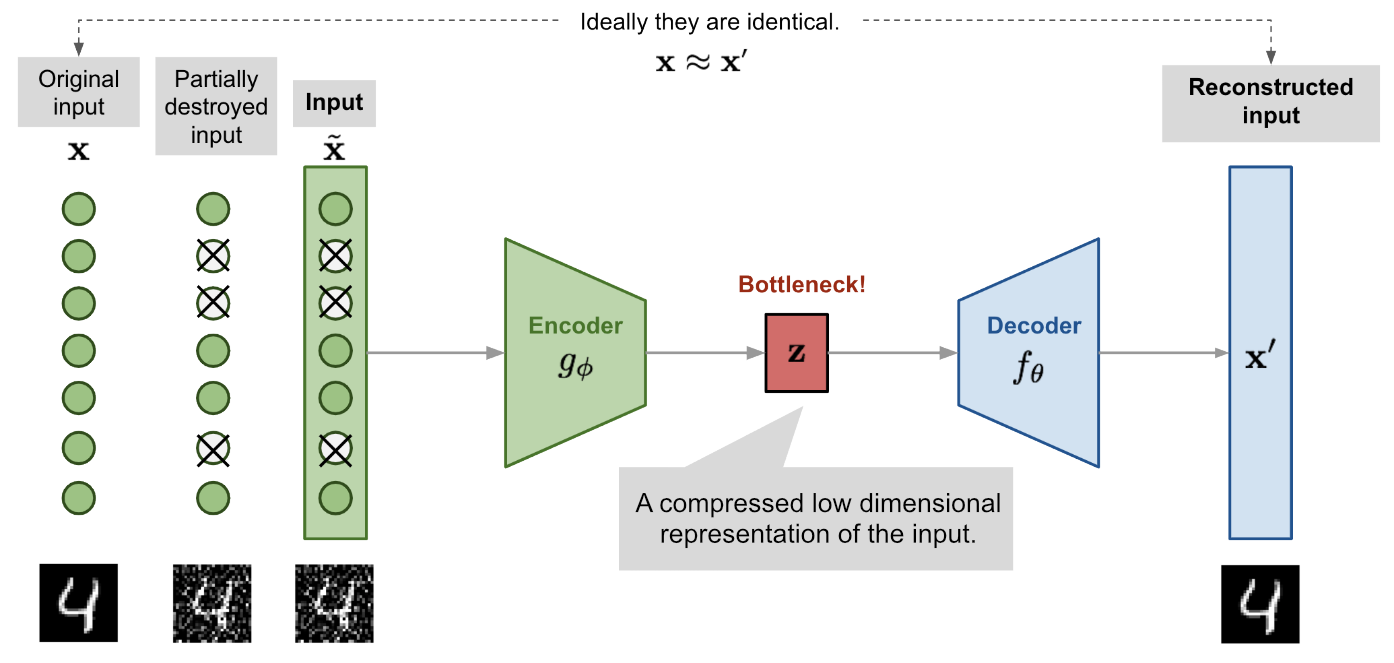
\includegraphics[width=0.95\linewidth]{gfx/denoising-autoencoder-architecture.png}
        \caption{Illustration of Denoising \acl{AE} model architecture, reproduced
        from \citet{wengAutoencoderBetaVAE2018}. \textit{Note: this figure uses
        the convention $f_{\theta}$ for the decoder and $g_{\phi}$ for the encoder,
        which is the reverse of the notation adopted in this thesis.}}
        \label{fig:denoising-ae}
    \end{figure}

    This design is motivated by the fact that humans can easily recognize an
    object or a scene even the view is partially occluded or corrupted. To
    ``repair'' the partially destroyed input, the denoising autoencoder has to
    discover and capture relationship between dimensions of input in order to
    infer missing pieces.

    For high dimensional input with high redundancy, like images, the model is
    likely to depend on evidence gathered from a combination of many input
    dimensions to recover the denoised version rather than to overfit one
    dimension. This builds up a good foundation for learning \textit{robust}
    latent representation.

    The noise is controlled by a stochastic mapping
    $\mathcal{M}_{\mathcal{D}}(\vb{x}_{c} \mid \vb{x})$, and it is not specific
    to a particular type of corruption process (\ie masking noise, Gaussian
    noise, salt-and-pepper noise, etc.). Naturally the corruption process can be
    equipped with prior knowledge \cite{wengAutoencoderBetaVAE2018}.

    \paragraph{Anomaly detection} \citet{sakuradaAnomalyDetectionUsing2014} were
    among the first to explicitly propose autoencoders as a tool for anomaly
    detection. Their core insight is that an autoencoder trained on normal data
    learns a compressed representation of the normal data distribution; at test
    time, inputs that deviate from this distribution are reconstructed poorly,
    and the resulting reconstruction error serves as an anomaly score. To
    substantiate this claim, they apply autoencoders to both synthetic data
    generated from the Lorenz system and real spacecraft telemetry, comparing
    against linear PCA and kernel PCA. They demonstrate that autoencoders, by
    virtue of their nonlinear dimensionality reduction, are able to detect
    subtle anomalies that linear PCA misses, while remaining computationally
    lighter than kernel PCA. This work established reconstruction error as a
    natural unsupervised anomaly signal for autoencoder-based methods.



\subsection{Sparse AutoEncoders} \label{sec:background:as:sae}

\acp{SAE} are one of the main variants of \ac{AE}. Just like \acp{AE}, they
learn a dictionary of feature directions from the input data, but they tipically
are overcomplete ($m \gg n$) and their latent representation is forced to be
sparse using some kind of sparsity mechanism. Given input $\vb{x} \in \R^{n}$,
the \ac{SAE} encodes it as:
\begin{equation*}
    \vb{z} = \operatorname{ReLU}(\vb{W}_{e}(\vb{x} - \vb{b}_{\mathrm{pre}}) +
    \vb{b}_{e}),
\end{equation*}
where $\vb{W}_{e} \in \R^{m \times n}$ is the encoder weight matrix,
$\vb{b}_{e} \in \R^{m}$ is the encoder bias, and $\vb{b}_{\mathrm{pre}} \in
\R^{n}$ is a pre-encoder bias subtracted from the input before encoding. This
learned offset allows the encoder to operate on roughly mean-centered
activations, improving training stability
\cite{brickenMonosemanticityDecomposingLanguage2023}. The decoder then
reconstructs the input as:
\begin{equation*}
    \hat{\vb{x}} = \vb{W}_{d} \vb{z} + \vb{b}_{\mathrm{pre}},
\end{equation*}
where $\vb{W}_{d} \in \R^{n \times m}$ is the decoder weight matrix. Each column
$\vb{d}_{i}$ of $\vb{W}_{d}$ is a dictionary atom, representing a candidate
feature direction in activation space.

When used in the context of \ac{MI}, the overcompleteness and the sparsity
constraint are motivated by the \textit{superposition hypothesis}.

\subsubsection{The Superposition Hypothesis}
\label{sec:background:ae:superposition}

A central challenge in \ac{MI} is that individual neurons in neural networks
tend to be \textit{polysemantic}: they activate in response to multiple,
seemingly unrelated concepts
\cite{elhageToyModelsSuperposition2022,olahZoomIntroductionCircuits2020}. An
example of this can be seen in
\cref{fig:polysemanticity}.
This runs contrary to the intuition that an interpretable model should have
neurons with clean, well-defined roles.

\begin{figure}[tb]
    \centering
    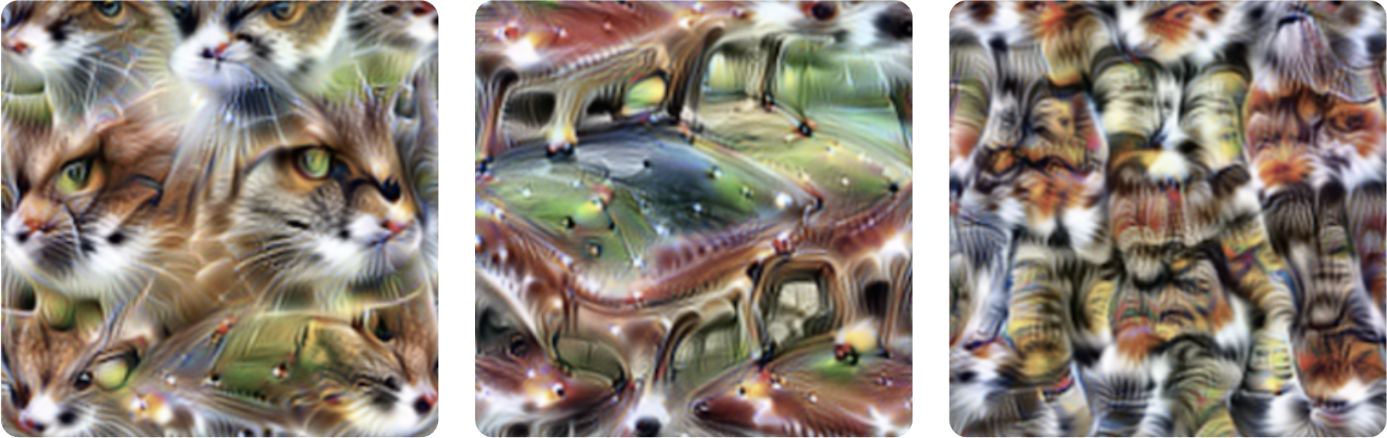
\includegraphics[width=0.95\linewidth]{gfx/polysemanticity.png}
    \caption{Neuron 4e:55, a polysemantic neuron from InceptionV1 which responds
    to cat faces, fronts of cars, and cat legs
    \cite{olahZoomIntroductionCircuits2020}.}
    \label{fig:polysemanticity}
\end{figure}

\citet{elhageToyModelsSuperposition2022} proposed the \textit{superposition
hypothesis} to explain this phenomenon. The core idea is that a network may
represent more features than it has dimensions, by exploiting the fact that
natural inputs are sparse: at any given time, only a small fraction of all
possible features are relevant. Under this condition, a network can pack many
near-orthogonal feature directions into a lower-dimensional space with limited
interference; polysemanticity ceases to be a failure of the model, and instead
becomes a rational compression strategy under capacity constraints.

This has a direct implication for interpretability: the natural basis of a
model's activations is not the neuron basis, but a larger, overcomplete set of
feature directions embedded within it. Recovering this basis requires moving
beyond individual neuron analysis, towards methods that can identify sparse,
distributed structure. This is precisely the goal of \textit{sparse dictionary
learning} \cite{olshausenSparseCodingOvercomplete1997}, a classical technique
from computational neuroscience that \acp{SAE} adapt to the setting of modern
language models.

\subsubsection{Architectures} \label{sec:background::ae:sae:arch}
There are many ways to enforce sparsity, each with its pros and cons. Here is a
selection of methods that range from the initial \ac{SAE} idea to more modern
architectures that try to improve on it.

    \paragraph{Vanilla $\ell_{1}$} This is the original architecture proposed by
    \citet{hubenSparseAutoencodersFind2023}. It uses an $\ell_{1}$\footnote{The
    $\ell_{p}$ norm is defined as $\ell_{p}(\vb{x}) = \norm{\vb{x}}_{p} =
    \left(\sum_{i} \abs{x_{i}}^{p}\right)^{\flatfrac{1}{p}},\ p \ge 1$.}
    penalty on the latent code to encourage most of $\vb{z}$'s entries to be
    exactly zero, so that any given activation is reconstructed from a small
    number of active features. The loss used to train this model is the
    following:
    \begin{equation*}
        \mathcal{L} = \norm{\vb{x} - \hat{\vb{x}}}^{2}_{2} + \lambda
        \norm{\vb{z}}_{1}.
    \end{equation*}
    The scalar $\lambda$ controls the sparsity--reconstruction trade-off and
    must be tuned carefully: too large, and reconstruction degrades; too small,
    and the learned features lose monosemanticity. A known side effect of
    $\ell_{1}$ regularisation is \textit{shrinkage}
    \cite{wrightAddressingFeatureSuppression2024,
    tibshiraniRegressionShrinkageSelection1996}: beyond driving inactive
    features to zero, the penalty also biases active feature magnitudes below
    their reconstruction-optimal values, causing the model to systematically
    underestimate the true activation of each feature
    \cite{rajamanoharanImprovingSparseDecomposition2024,
    wrightAddressingFeatureSuppression2024}. Constraining the decoder columns to
    unit $\ell_{2}$ norm after each gradient step partially mitigates this, by
    preventing the model from reducing the $\ell_{1}$ penalty through the
    trivial reparameterisation of scaling down encoder outputs and compensating
    with larger decoder norms
    \cite{rajamanoharanImprovingSparseDecomposition2024}. There is, however, a
    residual gradient-level bias that is structurally entangled with the
    $\ell_{1}$ penalty and can't be resolved with this trick.

    \paragraph{TopK SAEs} \citet{gaoScalingEvaluatingSparse2024} proposed
    replacing the $\ell_{1}$ penalty with a hard sparsity constraint,
    implemented via a TopK activation function that retains only the $k$ largest
    pre-activations and zeros the rest. This directly controls the number of
    active features per forward pass, eliminating the need to tune $\lambda$ and
    removing the shrinkage bias entirely. The full training objective is:
    \begin{equation*}
        \mathcal{L} = \norm{\vb{x} - \hat{\vb{x}}}^{2}_{2} + \alpha
        \mathcal{L}_{\mathrm{aux}},
    \end{equation*}
    where the auxiliary loss $\mathcal{L}_{\mathrm{aux}}$ addresses the problem
    of dead latents, \ie features that cease to activate entirely during
    training. Latents are flagged as dead if they have not activated for a
    predetermined number of tokens. Given the reconstruction residual $\vb{e} =
    \vb{x} - \hat{\vb{x}}$, the top-$k_{\mathrm{aux}}$ dead latents are selected
    and used to reconstruct $\vb{e}$; the resulting reconstruction error is
    $\mathcal{L}_{\mathrm{aux}}$. This gives dead latents a gradient signal
    proportional to how much of the residual they could explain, encouraging
    them to activate rather than remain permanently dormant.
    \citet{gaoScalingEvaluatingSparse2024} demonstrate that TopK \acp{SAE}
    achieve better reconstruction at equivalent sparsity levels compared to
    $\ell_{1}$ baselines, making them a strong and widely used alternative.

    \paragraph{Gated SAEs} \citet{rajamanoharanImprovingSparseDecomposition2024}
    introduced an architecture that separates the decision of whether a feature
    is active from the decision of how strongly it activates. A dedicated gating
    pathway produces a binary mask via a Heaviside step function (approximated
    during training with a straight-through estimator) which is applied
    element-wise to the encoder output. This architectural separation allows the
    model to learn feature presence and magnitude more independently, addressing
    shrinkage from a structural rather than a loss-based perspective.

    \paragraph{JumpReLU SAEs} \citet{rajamanoharanJumpingAheadImproving2024}
    proposed replacing the standard ReLU with a JumpReLU activation, which is
    zero below a learned per-feature threshold $\theta_{i}$ and equal to the
    pre-activation above it:
    \begin{equation*}
        \operatorname{JumpReLU}_{\theta_{i}}(z_{i}) = z_{i} \cdot \mathds{1}[z_{i} >
        \theta_{i}].
    \end{equation*}

    The key advantage of this parameterisation is that it provides a dedicated,
    per-feature learnable threshold, which allows the $\ell_{0}$ norm of the
    feature activations --- $\sum_{i} H(\pi_{i} - \theta_{i})$, where $\pi_{i}$
    are the encoder pre-activations and $H(x) = \mathds{1}[x > 0]$ is the
    Heaviside step function --- to be trained directly via a straight-through
    estimator applied to the threshold parameter $\theta_{i}$. Because each
    threshold can be positioned near the actual boundary between active and
    inactive pre-activations for its feature, the gradient signal is stable and
    controllable, making $\ell_{0}$ training practical in a way that would not
    be possible with a fixed threshold. Training with $\ell_{0}$ rather than
    $\ell_{1}$ eliminates shrinkage entirely, since $\ell_{0}$ penalises only
    the number of active features and not their intensity. JumpReLU \acp{SAE}
    achieve performance competitive with TopK \acp{SAE}.

\subsubsection{Application to Mechanistic Interpretability}
\label{sec:background:ae:sae:mechint}

The primary application of \acp{SAE} in \ac{MI} is \textit{feature discovery}:
training \iac{SAE} on the internal activations of a language model and examining
the resulting dictionary atoms to identify human-interpretable concepts. The
underlying hypothesis is that each dictionary atom, being active for only a
semantically coherent set of inputs, corresponds to a monosemantic feature of
the model's computation, a clean unit of meaning that the model had obscured in
the neuron basis.

\paragraph{Where SAEs are applied} \acp{SAE} can be trained on activations from
any layer or component of a transformer. \graffito{Make sure to mention what the
residual stream, \acs{MLP}, and attention heads are in a chapter about
\acsp{LLM}} Common targets include the residual stream at various depths,
\ac{MLP} layer outputs, and attention head outputs
\cite{hubenSparseAutoencodersFind2023,
brickenMonosemanticityDecomposingLanguage2023}. Each choice decomposes a
different aspect of the model's representations, and the resulting features
reflect the computational role of the targeted component. \graffito{Do we have a
reference for this?} Residual stream \acp{SAE}, for instance, tend to capture
more semantic, higher-level structure, while \ac{MLP}-targeted \acp{SAE} often
recover features more directly tied to knowledge retrieval and factual
associations.

\paragraph{Feature interpretability} In practice, learned features often
correspond to recognisable concepts.
\citet{brickenMonosemanticityDecomposingLanguage2023} trained \iac{SAE} on the
\ac{MLP} of a one-layer transformer and found features responsive to specific
tokens, syntactic roles, and semantic categories. Scaling this approach to
production-scale models, \citet{templetonScalingMonosemanticityExtracting} claim
to have identified lots of interpretable features, including neurons
representing famous people or countries, emotions, or even biases (racism,
sexism, hatred) and sarcastic praise. These results provide strong empirical
support for the superposition hypothesis and suggest that \acp{SAE} can serve as
a practical lens through which to study what information \acp{LLM} represent.

\paragraph{Evaluation} Assessing the quality of learned features is non-trivial,
as interpretability is inherently subjective. Several proxy metrics are used in
practice. \textit{Reconstruction quality} is typically measured by the
downstream \ac{CE} loss \graffito{Could this be made clearer?} recovered when
replacing original activations with \ac{SAE} reconstructions
\cite{gaoScalingEvaluatingSparse2024}. \textit{Sparsity} is quantified via the
average $\ell_{0}$ norm of the latent codes, \ie the mean number of active
features per token. \textit{Automated interpretability} pipelines use a second
language model to generate and score natural-language descriptions of individual
features \cite{billsLanguageModelsCan2023}, providing a scalable if imperfect
proxy for human judgement.

The inherent tension between these metrics -- reconstruction quality, sparsity,
and interpretability -- is a recurring theme in \ac{SAE} literature, and
motivates both the architectural variants described in
\cref{sec:background::ae:sae:arch}
and the alternative approach developed in this thesis and
described in \cref{sec:methods:model}.


\subsection{VAEs} \label{sec:background:ae:vae}
% \lipsum[1-3]
    \subsubsection{Architectures} \label{sec:background:ae:vae:arch}
        \paragraph{$\beta$-VAE}
        % \lipsum[1-3]
        \paragraph{VQ-VAE}
        % \lipsum[1-3]
    \subsubsection{Usage} \label{sec:background:ae:vae:usage}
        \paragraph{Generative model}
        % \lipsum[1-2]
        \paragraph{XAI}
        % \lipsum[1-2]

\section*{Conclusions}
% \lipsum[1]




%*****************************************
%*****************************************
%*****************************************
%*****************************************
%*****************************************
